\documentclass[fleqn]{article}
\usepackage[spanish,es-noshorthands]{babel}
\usepackage[utf8]{inputenc} 
\usepackage[papersize={6.5in,8.5in},total={5.5in,7.25in},centering]{geometry}
\usepackage{mathexam}
\usepackage{amsmath}
\usepackage{graphicx}
\usepackage{multicol}
\usepackage{tikz}

\ExamClass{
\includegraphics[height=16pt]{Images/logo-sed.png} Matemáticas $11^{\circ}$}
\ExamName{Nivelación 2}
\ExamHead{
\includegraphics[height=16pt]{Images/logo-colegio.png} IEDAB}
\newcommand{\LineaNombre}{%
\par
\vspace{\baselineskip}
Nombre:\hrulefill \; Curso: \underline{\hspace*{48pt}} \; Fecha: \underline{\hspace*{2.5cm}} \relax
\par}
\let\ds\displaystyle

\begin{document}
\ExamInstrBox{
Respuesta sin justificar mediante procedimiento no será tenida en cuenta en la calificación. Escriba sus procedimientos al respaldo o en una hoja anexa y sus respuestas en el espacio indicado o en una hoja anexa y las últimas 5, en el cuadro de respuestas que está al final. Tiene 45 minutos para contestar esta prueba.}
\LineaNombre
\begin{enumerate}
 \item Halle la distancia entre los números $-7$ y 8 usando como herramienta el valor absoluto y determine el punto medio.\noanswer
 \item Ubique en un plano cartesiano los puntos $A(-2,-5)$, $B(3,7)$, $C(-5,3)$ y $D(3,-5)$ y halle la distancia $\overline{AB}$
  \item Sabiendo que la ecuación estandard de la circunferencia de radio $r$, centrada en el punto $(h,k)$ es $(x-h)^{2}+(y-k)^{2}=r^{2}$, determine la ecuación standard de la circunferencia cuyo centro es el punto $(2,-4)$ y de radio $r=5$ \noanswer
 \item Teniendo en cuenta el siguiente gráfico
 \begin{center}
 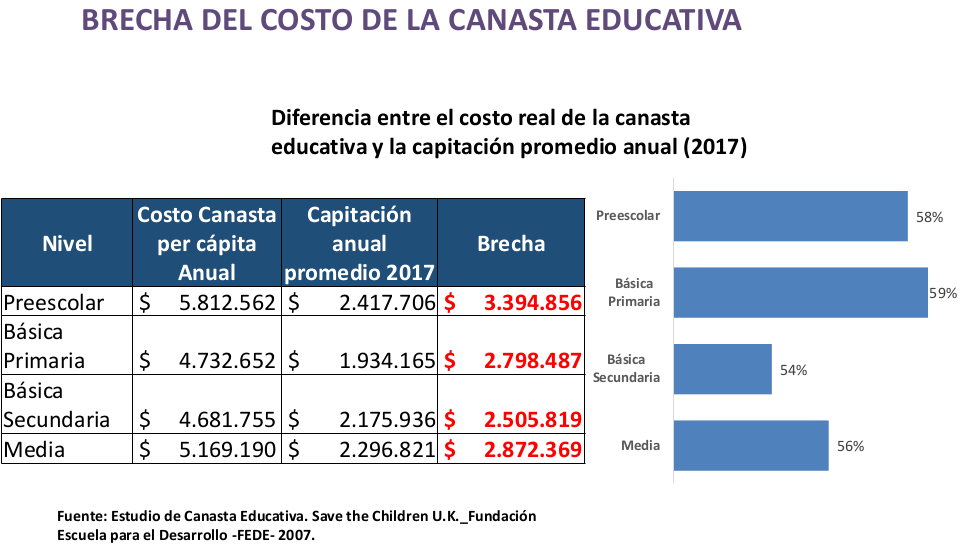
\includegraphics[scale=.375]{Images/BrechaCanasta.png} 
 \end{center}
 Conteste.
 \begin{enumerate}
 \item El estudio presentado en esta gráfica dice que para educar en condiciones apropiadas a un niño en primaria se necesitan \$4'732\,652 y en el año 2017 se invirtieron realmente \$1'934\,165 por estudiante. ¿Será que con un déficit de \$2'798\,487 se podrá brindar una educación digna?
 \item Determine a que corresponde el porcentaje que aparece a la derecha del gráfico. Hágalo por ejemplo para la educación media (56\%), verificando con la operación respectiva \noanswer
 \end{enumerate}
 \item Construya las primeras 7 filas del triángulo de Pascal. Con base en éste, calcule \noanswer
 \begin{enumerate}
 \begin{multicols}{3}
 \item $\displaystyle{7 \choose 2}$
 \item $\displaystyle{7 \choose 4}$
 \item $\displaystyle{7 \choose 3}$
 \end{multicols}
 \end{enumerate}
 \item ¿Cuál de las siguientes opciones es el punto medio del segmento de recta con extremos $-6$ y 3? Justifique su respuesta
 \begin{enumerate}
 \begin{multicols}{5}
 \item $4/2$
 \item 4.3
 \item $-1/2$
 \item $-3/2$
  \item $-6/2$
 \end{multicols}
 \end{enumerate}
 \item ¿Cuál de las siguientes opciones es el centro de la circunferencia $(x+5)^{2}+(y-6)^{2}=16$?
 \begin{enumerate}
 \begin{multicols}{5}
 \item $(-5,-6)$
 \item $(-6,5)$
 \item $(6,-5)$
  \item $(5,-6)$
   \item $(-5,6)$
 \end{multicols}
 \end{enumerate}
 \item Si la distancia entre dos puntos A y B de una recta numérica no es menor que 3, la gráfica que representa dos puntos con esta condición es:

\begin{enumerate}
\item 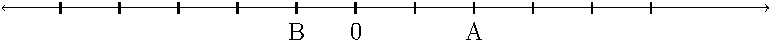
\includegraphics[scale=.5]{Images/respA.pdf}
\item 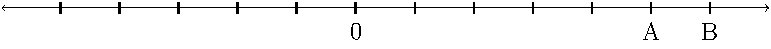
\includegraphics[scale=.5]{Images/respC.pdf} 
\item 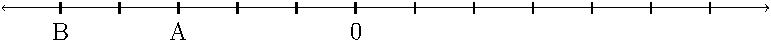
\includegraphics[scale=.5]{Images/respD.pdf} 
\item 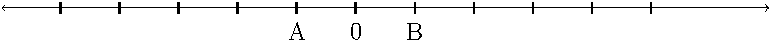
\includegraphics[scale=.5]{Images/respB.pdf} 
\end{enumerate}
 \item ¿Cuál de los siguiente números NO aparece en el octavo renglón del triángulo de Pascal
 \begin{enumerate}
 \begin{multicols}{5}
 \item 28
 \item 9
 \item 70
  \item 1
   \item 56
 \end{multicols}
 \end{enumerate}
 \item $(x+y)^{3}-(x-y)^{3}=$
 \begin{enumerate}
 \begin{multicols}{5}
 \item $-2y^{3}$
  \item $6x^{2}y+2y^{3}$
 \item $2x^{3}+6xy^{2}$
 \item $6xy^{2}+2y^{3}$
  \item $2x^{3}$
 \end{multicols}
 \end{enumerate}
 \end{enumerate}
 \begin{center}
\begin{tabular}{cccccccccccc}
6 & 7 & 8 & 9 & 10 \\ 
\textcircled{a} & \textcircled{a} & \textcircled{a} & \textcircled{a} & \textcircled{a}\\ 
\textcircled{b} & \textcircled{b} & \textcircled{b} & \textcircled{b} & \textcircled{b} \\ 
\textcircled{c} & \textcircled{c} & \textcircled{c} & \textcircled{c} & \textcircled{c}\\ 
\textcircled{d} & \textcircled{d} & \textcircled{d} & \textcircled{d} & \textcircled{d} \\ 
\textcircled{e} & \textcircled{e} & \textcircled{e} & \textcircled{e} & \textcircled{e}\\
\end{tabular} 
\end{center}
\end{document}
